\section{动画变换}\label{sec:动画变换}
\begin{remark}
    本节含有高级内容,第一次阅读时可以跳过。
\end{remark}

\begin{figure}[htbp]
    \centering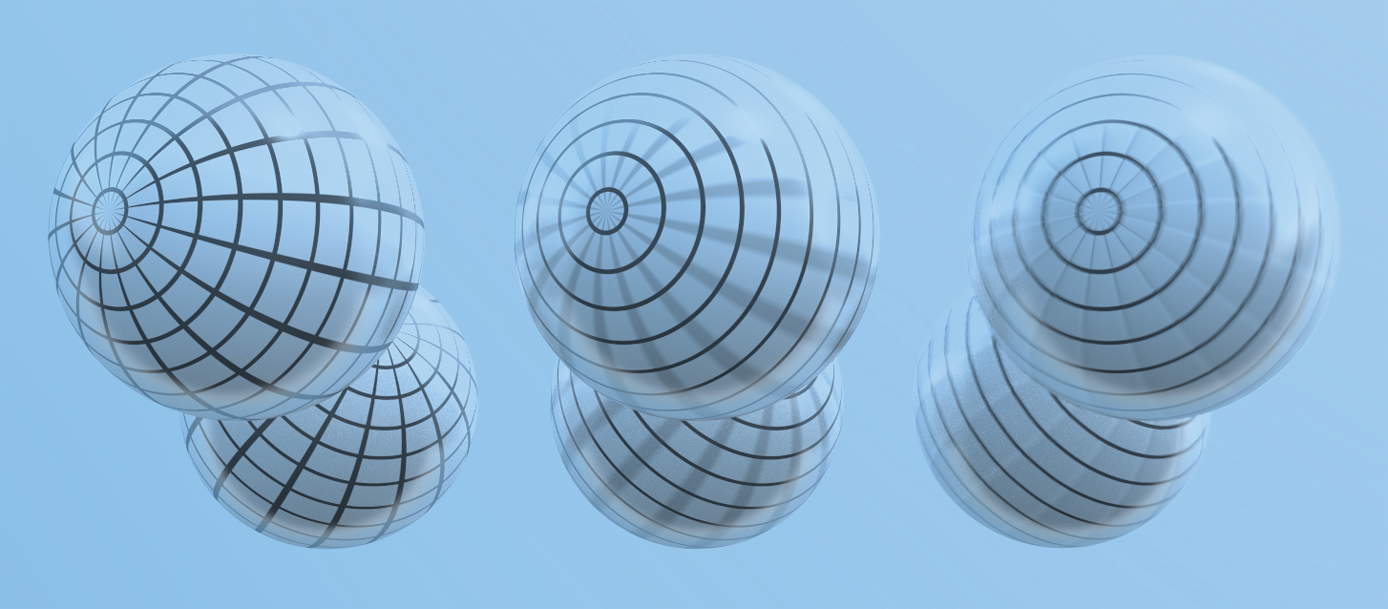
\includegraphics[width=\linewidth]{chap02/spinningspheres.png}
    \caption{转动的球体。用本节实现的变换动画代码以不同速率旋转三个球体并被镜子反射。
        注意球体的反射和球体自身一样模糊。}
    \label{fig:2.15}
\end{figure}

pbrt为场景中的相机和几何图元支持关键帧矩阵动画。
不只是提供单个变换放置场景中的相应物体,
用户还可能提供许多\keyindex{关键帧}{keyframe}{}变换,
每个都与特定时间点关联。
这能让相机移动起来并在仿真相机快门打开时让场景中的物体也移动起来。
\reffig{2.15}展示了三个运用pbrt关键帧矩阵动画的运动球体。

通常,在关键帧矩阵之间插值的问题是没有定义的。
例如,如果我们关于$x$轴旋转181度后再旋转181度,
这代表2度的小旋转还是-358度的大旋转?
再例如,考虑两个矩阵,一个是恒等的另一个是绕$z$轴旋转180度。
从其中一个到另一个有无数种方式可走。

关键帧矩阵插值在计算机动画中是一个重要的问题,
有许多不同的方法被开发出来。
幸运的是,有两个原因使得渲染器中的矩阵插值问题一般不像动画系统中的那么难。

首先,在一个像pbrt那样的渲染器中,
我们一般有分别在相机快门打开和关闭时的关键帧矩阵;
我们只需要在单张图像的时段里在两者之间插值。
在动画系统中,矩阵一般按更低的时间频率提供,
所以一对关键帧矩阵之间有许多帧;
这样,就有更多机会注意到插值中的问题。

第二,在基于物理的渲染器中,需要我们插值的矩阵对的时段越长,
虚拟相机快门就打开得越久,最终图像的运动模糊就越多;
运动模糊的增加常常隐藏了插值的缺点。

对由关键帧矩阵定义的变换最简单的插值方法——
直接对矩阵的每个分量插值——并不是一个好办法,因为它一般会导致意外不良结果。
例如,如果变换应用了不同的旋转,则即使是刚体运动,中间的矩阵也可能缩放物体,这明显不是我们期望的。
(如果矩阵在它们之间有完整180度的旋转,则插值的中间物体可能缩小到不见!)

\reffig{2.16}展示了在该帧过程中旋转90度的球体;
直接对矩阵元素插值给出的结果不如本节实现的方法准确。
\begin{figure}[htbp]
    \raggedright
    \subfloat[静止球体。]{\label{fig:2.16.1}
\includegraphics[width=0.5\linewidth]{chap02/sphere-still.png}}%
    \subfloat[旋转,正确插值。]{\label{fig:2.16.2}
\includegraphics[width=0.5\linewidth]{chap02/sphere-rot-good.png}}\\%
    \subfloat[旋转,错误插值。]{\label{fig:2.16.3}
\includegraphics[width=0.5\linewidth]{chap02/sphere-rot-bad.png}}\quad%
    \begin{minipage}{0.45\textwidth}
        \vspace{-\linewidth}\caption{变换插值错误的影响。(a)球体以网格线作为纹理,没有旋转。
            (b)球体在该帧过程中旋转90度,使用本节实现的变换插值技术。
            (c)球体旋转90度,直接对矩阵分量插值来对变换插值。
            这时,动画球体错误地变大了并且靠球体外本应清晰的线条也错误地变模糊了。}
        \label{fig:2.16}
    \end{minipage}
\end{figure}

pbrt中使用的变换插值方法是基于\keyindex{矩阵分解}{matrix decomposition}{}——
给定任意变换矩阵$\bm M$,我们将其分解为
缩放($\bm S$)、旋转($\bm R$)和平移($\bm T$)变换的级联,
\begin{align*}
    \bm M=\bm S\bm R\bm T\, ,
\end{align*}
其中这些分量每一个都是独立插值,然后合成的插值矩阵由三个插值矩阵一起相乘得到。

平移和缩放的插值可以由矩阵分量的线性插值轻松准确完成;
旋转插值则更困难。
在描述pbrt中的矩阵分解实现之前,我们首先介绍\keyindex{四元数}{quaternion}{},
它对旋转的优雅表示将给出高效的插值方法。

\subsection{四元数}\label{sub:四元数}
四元数\sidenote{译者注:本节内容对四元数的介绍比较精简,不加证明地给出相关性质。
    如果你关心这些性质背后的原因是什么,可以阅读译者自行整理编写的\refsec{译者补充:四元数}。}
作为复数的推广,最初由William Rowan Hamilton爵士于1843年发明。
就像复数可以定义为实部和虚部之和$x+y\mathbf{i}$,其中$\mathbf{i}^2=-1$那样,
他确定也能推广到四维,得到了四元数。

四元数是一个四元组,
\begin{align}\label{eq:2.4}
    \bm q=(x,y,z,w)=w+x\mathbf{i}+y\mathbf{j}+z\mathbf{k}\, ,
\end{align}
其中$\mathbf{i}, \mathbf{j}, \mathbf{k}$定义
\footnote{Hamilton发现分量之间的这种关系非常有趣,
    以至于当他想到这个时立即用刀子把公式刻在了他正经过的桥上。}
为$\mathbf{i}^2=\mathbf{j}^2=\mathbf{k}^2=\mathbf{i}\mathbf{j}\mathbf{k}=-1$。
分量间的另一重要关系是$\mathbf{i}\mathbf{j}=\mathbf{k}$且
$\mathbf{j}\mathbf{i}=-\mathbf{k}$。
这说明四元数乘法一般是不可交换的。

四元数可以表示为四元组$\bm q=(q_x,q_y,q_z,q_w)$或$(\bm q_{xyz},q_w)$,
其中$\bm q_{xyz}$是虚部三维向量,$q_w$是实部。
本节中我们会穿插使用这两种表示。

两个任意四元数的乘积表达式可以通过展开它们定义的实部和虚部得到:
\begin{align*}
    \bm q\bm q'=(q_w+q_x\mathbf{i}+q_y\mathbf{j}+q_z\mathbf{k})(q'_w+q'_x\mathbf{i}+q'_y\mathbf{j}+q'_z\mathbf{k})\, .
\end{align*}

整理各项并利用像上面列出的分量间恒等式(例如$\mathbf{i}^2=-1$),
结果可用向量叉积和点积简洁地表示为
\begin{align}\label{eq:2.5}
    (\bm q\bm q')_{xyz} & =\bm q_{xyz}\times\bm q'_{xyz}+q_w\bm q'_{xyz}+q'_w\bm q_{xyz}\nonumber\, , \\
    (\bm q\bm q')_w     & =q_wq'_w-(\bm q_{xyz}\cdot\bm q'_{xyz})\, .
\end{align}

单位四元数(分量满足$x^2+y^2+z^2+w^2=1$的四元数)和
$\mathbb{R}^3$空间中的旋转之间有一很有用的关系:具体来说,
绕着可以映射为单位四元数$(\hat{\bm v}\sin\theta,\cos\theta)$的
单位轴$\hat{\bm v}$旋转角度$2\theta$时,
下列四元数乘积等效于将旋转施加到点$\bm p$后表达为齐次坐标形式:
\begin{align*}
    \bm p'=\bm q\bm p\bm q^{-1}\, .
\end{align*}

并且,若干旋转四元数的积得到的另一个四元数等价于依次施加旋转。

pbrt中文件\href{https://github.com/mmp/pbrt-v3/tree/master/src/core/quaternion.h}{{\ttfamily core/quaternion.h}}
和\href{https://github.com/mmp/pbrt-v3/tree/master/src/core/quaternion.cpp}{{\ttfamily core/quaternion.cpp}}
中有类\refvar{Quaternion}{}
的实现。默认构造函数初始化一个单位四元数。
\begin{lstlisting}
`\initcode{Quaternion Public Methods}{=}\initnext{QuaternionPublicMethods}`
`\initvar{Quaternion}{}`() : `\refvar[Quaternion::v]{v}{}`(0, 0, 0), `\refvar[Quaternion::w]{w}{}`(1) { }
\end{lstlisting}

我们用\refvar{Vector3f}{}表示四元数的$xyz$分量;
这样可以在下面一些方法的实现中利用\refvar{Vector3f}{}的各种方法。
\begin{lstlisting}
`\initcode{Quaternion Public Data}{=}`
`\refvar{Vector3f}{}` `\initvar[Quaternion::v]{v}{}`;
`\refvar{Float}{}` `\initvar[Quaternion::w]{w}{}`;
\end{lstlisting}

四元数的加减法逐元素执行。这直接由\refeq{2.4}推导而来。例如
\begin{align*}
    \bm q+\bm q' & =(w+x\mathbf{i}+y\mathbf{j}+z\mathbf{k})(w'+x'\mathbf{i}+y'\mathbf{j}+z'\mathbf{k})\nonumber \\
                 & =(w+w')+(x+x')\mathbf{i}+(y+y')\mathbf{j}+(z+z')\mathbf{k}\, .
\end{align*}

其他算术方法(减法、乘法以及除以标量)也有类似定义和实现,此处不再赘述。
\begin{lstlisting}
`\refcode{Quaternion Public Methods}{+=}\lastnext{QuaternionPublicMethods}`
`\refvar{Quaternion}{}` &operator+=(const `\refvar{Quaternion}{}` &q) {
    `\refvar[Quaternion::v]{v}{}` += q.`\refvar[Quaternion::v]{v}{}`;
    `\refvar[Quaternion::w]{w}{}` += q.`\refvar[Quaternion::w]{w}{}`;
    return *this;
}
\end{lstlisting}

两个四元数的内积由方法\refvar[Quaternion::Dot]{Dot}{()}实现,
并且四元数可以被它的长度规范化。
\begin{lstlisting}
`\initcode{Quaternion Inline Functions}{=}\initnext{QuaternionInlineFunctions}`
inline `\refvar{Float}{}` `\initvar[Quaternion::Dot]{Dot}{}`(const `\refvar{Quaternion}{}` &q1, const `\refvar{Quaternion}{}` &q2) {
    return `\refvar{Dot}{}`(q1.`\refvar[Quaternion::v]{v}{}`, q2.`\refvar[Quaternion::v]{v}{}`) + q1.`\refvar[Quaternion::w]{w}{}` * q2.`\refvar[Quaternion::w]{w}{}`;
}
\end{lstlisting}

\begin{lstlisting}
`\refcode{Quaternion Inline Functions}{+=}\lastcode{QuaternionInlineFunctions}`
inline `\refvar{Quaternion}{}` `\initvar[Quaternion::Normalize]{Normalize}{}`(const `\refvar{Quaternion}{}` &q) {
    return q / std::sqrt(`\refvar[Quaternion::Dot]{Dot}{}`(q, q));
}
\end{lstlisting}

能够计算和四元数表示同一旋转的变换矩阵非常有用。特别地,在类
\refvar{AnimatedTransform}{}中用四元数对旋转插值后,
我们需要将插值后的旋转转换回变换矩阵来计算最后合成的插值矩阵。

为了推导四元数的旋转矩阵,回忆一下四元数对点的变换由$\bm q\bm p\bm q^{-1}$给出。
我们想要矩阵$\bm M$执行相同的变换,即$\bm p'=\bm M\bm p$。
如果我们用\refeq{2.5}展开四元数乘法$\bm q\bm p\bm q^{-1}$、
用四元数基本恒等式化简、合并项并把结果表示为矩阵,
我们可以得到如下$3\times3$矩阵表示同一变换:
\begin{align}\label{eq:2.6}
    \bm M=\left[
        \begin{array}{ccc}
            1-2(q_y^2+q_z^2) & 2(q_xq_y+q_zq_w) & 2(q_xq_z-q_yq_w) \\
            2(q_xq_y-q_zq_w) & 1-2(q_x^2+q_z^2) & 2(q_yq_z+q_xq_w) \\
            2(q_xq_z+q_yq_w) & 2(q_yq_z-q_xq_w) & 1-2(q_x^2+q_y^2)
        \end{array}
        \right]\, .
\end{align}

该计算由方法\refvar[ToTransform]{Quaternion::ToTransform}{()}实现。
我们此处不介绍它的实现,因为它就是\refeq{2.6}的直接实现。
\begin{lstlisting}
`\refcode{Quaternion Public Methods}{+=}\lastnext{QuaternionPublicMethods}`
`\refvar{Transform}{}` `\initvar{ToTransform}{}`() const;
\end{lstlisting}

注意我们可以利用一个单位四元数
$\displaystyle(\bm q_{xyz}\sin\frac{\theta}{2},\cos\frac{\theta}{2})$表示
绕单位轴$\hat{\bm q}_{xyz}$旋转角度$\theta$的事实计算旋转矩阵。
首先我们计算出旋转角度为$\theta=2\arccos q_w$,
然后利用之前定义的函数\refvar{Rotate}{()},
传入轴$\hat{\bm q}_{xyz}$和旋转角度$\theta$。
然而,这个替代方法会很低效,因为需要多次调用三角函数,
但是这里实现的方法只用了浮点加法、减法和乘法。

从旋转矩阵创建四元数也很有用。
为此,\refvar{Quaternion}{}提供了接收\refvar{Transform}{}
的构造函数。合适的四元数可以通过利用\refeq{2.6}中旋转矩阵元素与四元数分量之间的关系算得。
例如,如果我们从矩阵本身中减去它的转置,则结果矩阵的$(0,1)$分量为$-4q_wq_z$。
因此,给定已知值的特定旋转矩阵实例,
可以利用矩阵值与四元数分量之间大量这样的关系生成一系列可以求解四元数分量的方程。

本文中我们不介绍推导细节或实际实现
\sidenote{译者注:笔者将其补充到了\refsub{四元数与旋转变换}。};
关于怎样推导这项技术的更多信息,
包括处理数值稳定性,详见\citet{SHOEMAKE1991351}。

\begin{lstlisting}
`\refcode{Quaternion Public Methods}{+=}\lastcode{QuaternionPublicMethods}`
`\refvar{Quaternion}{}`(const `\refvar{Transform}{}` &t);
\end{lstlisting}

\subsection{四元数插值}\label{sub:四元数插值}
我们最后要定义的函数\refvar{Slerp}{()},
在两个四元数之间进行\keyindex{球面线性插值}{spherical linear interpolation}{interpolation插值}(slerp)。
球面线性插值可在球体表面大圆的弧线上做匀速率运动,
因此对于旋转插值有两个期望的性质:
\begin{itemize}
    \item 旋转插值路径使得\keyindex{扭矩最小化}{torque minimization}{}:
          两个旋转之间所得路径是旋转空间中所能得到的最短路径。
    \item 插值有\keyindex{恒定角速度}{constant angular velocity}{}:
          动画参数{\ttfamily t}的变化量和所得旋转的变化量的关系在插值过程中是恒定的
          (换句话说,在插值范围内,插值速度是恒定的)。
\end{itemize}

参考本章末“扩展阅读”一节更彻底地讨论好的旋转插值该有什么性质。

如下的四元数球面线性插值最初由\citet{10.1145/325334.325242}提出,
给定两个四元数$\bm q_1$和$\bm q_2$和参数值$t\in[0,1]$以在两者之间插值
\sidenote{译者注:利用三角形的正弦定理可以推导出该公式。}:
\begin{align*}
    \mathrm{slerp}(\bm q_1,\bm q_2,t)=\frac{\bm q_1\sin((1-t)\theta)+\bm q_2\sin(t\theta)}{\sin\theta}\, .
\end{align*}

\citet{Blow_2004}提出了一种直观的方式理解\refvar{Slerp}{()}。
下文中,给定要在其间插值的四元数$\bm q_1$和$\bm q_2$,两者角度记为$\theta$。
然后,给定参数值$t\in[0,1]$,我们想要找到中间的四元数$\bm q'$使得
它沿从$\bm q_1$到$\bm q_2$的路径与$\bm q_1$的角度为$\theta'=\theta t$。

\begin{figure}[htbp]
    \centering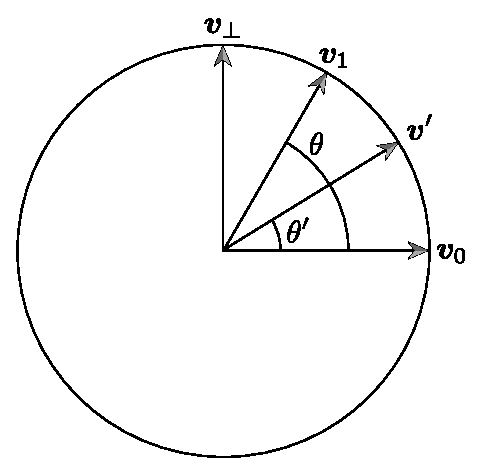
\includegraphics[scale=0.6]{chap02/Quaternionrotation.eps}
    \caption{为了理解四元数球面线性插值,考虑2D下的两个单位圆上的向量$\bm v_0$和$\bm v_1$,
        两者夹角$\theta$。我们想要计算两者间角度为$\theta'$的插值向量。
        为此,我们可以寻找正交于$\bm v_0$的向量$\bm v_{\perp}$,
        再应用三角恒等式$\bm v'=\bm v_0\cos\theta'+\bm v_{\perp}\sin\theta'$。}
    \label{fig:2.17}
\end{figure}

一个计算$\bm q'$的简单方法是先在四元数空间中计算一个正交坐标系统,
一个轴为$\bm q_1$,另一个是与$\bm q_1$正交的四元数,
这样两轴就构成张开$\bm q_1$和$\bm q_2$的基。

有了这个坐标系统,我们就能计算关于$\bm q_1$的旋转
(见\reffig{2.17}展示的2D设置下的概念)。
正交向量$\bm q_{\perp}$可以通过将$\bm q_2$投影到$\bm q_1$并
从$\bm q_2$减去该正交投影得到;
剩余部分保证与$\bm q_1$正交:
\begin{align}\label{eq:2.7}
    \bm q_{\perp}=\bm q_2-(\bm q_1\cdot\bm q_2)\bm q_1\, .
\end{align}
给定坐标系统和规范化的$\bm q_{\perp}$,沿动画路径的四元数为
\begin{align}\label{eq:2.8}
    \bm q'=\bm q_1\cos(\theta t)+\hat{\bm q}_{\perp}\sin(\theta t)\, .
\end{align}

函数\refvar{Slerp}{()}的实现检查看两个四元数是否几乎平行,
是的话它就按顺序对四元数分量用普通的线性插值以避免数值不稳定。
否则,它就用\refeq{2.7}计算正交四元数{\ttfamily qperp},
然后按\refeq{2.8}计算插值的四元数。
\begin{lstlisting}
`\initcode{Quaternion Method Definitions}{=}`
`\refvar{Quaternion}{}` `\initvar{Slerp}{}`( `\refvar{Float}{}` t, const `\refvar{Quaternion}{}` &q1,
                 const `\refvar{Quaternion}{}` &q2) {
     `\refvar{Float}{}` cosTheta = `\refvar[Quaternion::Dot]{Dot}{}`(q1, q2);
    if (cosTheta > .9995f)
        return `\refvar[Quaternion::Normalize]{Normalize}{}`((1 - t) * q1 + t * q2);
    else {
        `\refvar{Float}{}` theta = std::acos(`\refvar{Clamp}{}`(cosTheta, -1, 1));
        `\refvar{Float}{}` thetap = theta * t;
        `\refvar{Quaternion}{}` qperp = `\refvar[Quaternion::Normalize]{Normalize}{}`(q2 - q1 * cosTheta);
        return q1 * std::cos(thetap) + qperp * std::sin(thetap);
    }
}
\end{lstlisting}

\subsection{动画变换实现}\label{sub:动画变换实现}
给定

\begin{lstlisting}
`\initcode{AnimatedTransform Method Definitions}{=}\initnext{AnimatedTransformMethodDefinitions}`
`\initvar{AnimatedTransform}{}`::`\refvar{AnimatedTransform}{}`(const `\refvar{Transform}{}` *startTransform,
        `\refvar{Float}{}` startTime, const `\refvar{Transform}{}` *endTransform, `\refvar{Float}{}` endTime)
    : `\refvar{startTransform}{}`(startTransform), `\refvar{endTransform}{}`(endTransform),
      `\refvar{startTime}{}`(startTime), `\refvar{endTime}{}`(endTime),
      `\refvar{actuallyAnimated}{}`(*startTransform != *endTransform) {
    `\refvar{Decompose}{}`(startTransform->m, &`\refvar[AnimatedTransform::T]{T}{}`[0], &`\refvar[AnimatedTransform::R]{R}{}`[0], &`\refvar[AnimatedTransform::S]{S}{}`[0]);
    `\refvar{Decompose}{}`(endTransform->m, &`\refvar[AnimatedTransform::T]{T}{}`[1], &`\refvar[AnimatedTransform::R]{R}{}`[1], &`\refvar[AnimatedTransform::S]{S}{}`[1]);
    `\refcode{Flip R[1] if needed to select shortest path}{}`
    `\refvar{hasRotation}{}` = `\refvar[Quaternion::Dot]{Dot}{}`(`\refvar[AnimatedTransform::R]{R}{}`[0], `\refvar[AnimatedTransform::R]{R}{}`[1]) < 0.9995f;
    `\refcode{Compute terms of motion derivative function}{}`
}
\end{lstlisting}

\begin{lstlisting}
`\initcode{AnimatedTransform Private Data}{=}\initnext{AnimatedTransformPrivateData}`
const `\refvar{Transform}{}` *`\initvar{startTransform}{}`, *`\initvar{endTransform}{}`;
const `\refvar{Float}{}` `\initvar{startTime}{}`, `\initvar{endTime}{}`;
const bool `\initvar{actuallyAnimated}{}`;
`\refvar{Vector3f}{}` `\initvar[AnimatedTransform::T]{T}{}`[2];
`\refvar{Quaternion}{}` `\initvar[AnimatedTransform::R]{R}{}`[2];
`\refvar{Matrix4x4}{}` `\initvar[AnimatedTransform::S]{S}{}`[2];
bool `\initvar{hasRotation}{}`;
\end{lstlisting}